% CVPR 2026 Paper Template; see https://github.com/cvpr-org/author-kit

\documentclass[10pt,twocolumn,letterpaper]{article}

%%%%%%%%% PAPER TYPE  - PLEASE UPDATE FOR FINAL VERSION
\usepackage{cvpr}              % Camera-ready CVPR layout for the course report
% \usepackage[review]{cvpr}    % Review layout
% \usepackage[pagenumbers]{cvpr} % To force page numbers, e.g. for an arXiv version

% Import additional packages in the preamble file, before hyperref
%% This file contains a number of tweaks that are typically applied to the main document.
%% They are not enabled by default, but can be enabled by uncommenting the relevant lines.


%%
%% Official support for 2-column teaser figure
%%

%%
%% For auto-referencing of figures (see fig/teaser.tex and \label{} therein) 
%%

%%
%% caption and (global) spacing overrides
%%
% \setlength{\abovecaptionskip}{.5em} % space above caption
% \setlength{\belowcaptionskip}{1em} % space below caption

%%
%% Inline annotations; for predefined colors, refer to "dvipsnames" in the xcolor package:
%% https://tinyurl.com/overleaf-colors
%%
\newcommand{\red}[1]{{\color{red}#1}}
\newcommand{\todo}[1]{{\color{red}#1}}
\newcommand{\TODO}[1]{\textbf{\color{red}[TODO: #1]}}
%%
%% Disable for camera ready / submission by uncommenting these lines:
%%
% \renewcommand{\TODO}[1]{}
% \renewcommand{\todo}[1]{#1}

%%
%% Work harder in optimizing text layout. Typically shrinks text by 1/6 of page, enable
%% it at the very end of the writing process, when you are just above the page limit.
%%
% \usepackage{microtype}

%%
%% Fine-tune paragraph spacing.
%%
% \renewcommand{\paragraph}[1]{\vspace{.5em}\noindent\textbf{#1.}}

%%
%% Globally adjusts space between figure and caption.
%%
% \setlength{\abovecaptionskip}{.5em}

%%
%% Allows "the use of \paper to refer to the project name"
%% with automatic management of space at the end of the word.
%%
% \usepackage{xspace}
% \newcommand{\paper}{ProjectName\xspace}

%%
%% Commonly used math definitions.
%%
% \DeclareMathOperator*{\argmin}{arg\,min}
% \DeclareMathOperator*{\argmax}{arg\,max}

%%
%% Tighten underline.
%%
% \usepackage{soul}
% \setuldepth{foobar}

%%
%% Reconfigure paragraph (tweaks spacing)
%%


\definecolor{cvprblue}{rgb}{0.21,0.49,0.74}
\usepackage[pagebackref,breaklinks,colorlinks,allcolors=cvprblue]{hyperref}

%%%%%%%%% PAPER ID  - PLEASE UPDATE
\def\paperID{1}
\def\confName{CVPR}
\def\confYear{2026}

%%%%%%%%% TITLE - PLEASE UPDATE
\title{A Scene-Level Matcher for Two-View Amodal Object Association}

%%%%%%%%% AUTHORS - PLEASE UPDATE
\author{CIE6004 Project 1 Submission\\
Course Project Report
% For a paper whose authors are all at the same institution,
% omit the following lines up until the closing ``}''.
% Additional authors and addresses can be added with ``\and'',
% just like the second author.
% To save space, use either the email address or home page, not both
}

\begin{document}
\maketitle
\begin{abstract}
This report studies joint detection, cross-view association, and deduplicated counting for 200 paired tabletop scenes. A YOLO26n detector is fine-tuned on the supplied amodal boxes. For each pair of views, a learned scene-level matcher combines appearance, box shape, detection confidence, and camera-based ground-plane projection cues. It predicts links and unmatched options, then uses partial one-to-one assignment to form one record per object. On the labeled validation set, the selected system obtains 0.9805 detection F1, 0.9531 association F1, 0.9840 given-detection association F1, and a count MAE of 0.230 objects. A controlled comparison shows that scene-level context improves over a pairwise scorer, while camera-guided recovery raises detection recall but does not conclusively improve the combined association and counting trade-off. Test predictions are provided in the assignment format; test labels were not used.
\end{abstract}

\section{Introduction}
The task is to produce one record per physical package in a pair of images: each record contains a bounding box in view A and the corresponding box in view B. The boxes are amodal, the views have independent pixel coordinates, and the number of records is the deduplicated count. The primary score is cross-view association F1; detection F1 and per-scene count error are also graded \cite{coursebrief}. Thus, strong single-view detection is not sufficient: even two accurate boxes reduce association performance if they are assigned to different objects.

The images contain many visually similar packages and large viewpoint changes. We address this by separating candidate detection from scene-level matching. A fine-tuned YOLO26n model proposes boxes, and a compact learned matcher evaluates all candidate links jointly. It combines DINOv2 crop appearance, HSV color histograms, object-box shape, confidence, and a symmetric camera projection prior. Explicit unmatched scores allow the system to leave uncertain detections unpaired instead of forcing a complete matching.

The chosen configuration is the 960-pixel shared detector with the scene-level matcher and no low-confidence recovery. It has the best measured overall balance on validation. The recovery variant obtains a slightly higher association F1 point estimate, but its paired scene-bootstrap interval includes no change and its count metrics are lower. The report therefore treats it as a useful ablation rather than the selected system.

\section{Method}
\subsection{Amodal candidate detection}
The provided annotations mark the complete object extent, including occluded portions. A pretrained YOLO26n detector was fine-tuned for 80 epochs on the 1,000 labeled training scene pairs as a single object class. Training used 640-pixel input, batch size 16, seed 42, and the supplied training augmentation. The best detector checkpoint was selected by the Ultralytics validation mAP criterion. At inference, the same detector is applied independently to both views at image size 960, confidence 0.45, NMS IoU 0.6, and at most 40 boxes per image. Predicted coordinates are mapped back to the original 512 by 512 image grid. No test labels or manual test annotations are used.

\subsection{Pair features and scene-level matching}
For every candidate box in A and B, we compute ten pair features: the normalized A-to-B and B-to-A camera reprojection residuals, their disagreement, HSV-histogram cosine similarity, DINOv2 ViT-S/14 crop-feature cosine similarity, the two detector confidence scores, and log ratios for width, height, and area. DINOv2 is frozen and used only to extract crop descriptors; it is not fine-tuned \cite{dinov2}. Each box bottom-center is back-projected to the supplied orthographic table plane and projected into the opposite view. This cue is a soft location prior: amodal box geometry and object height mean it is not a reliable pixel correspondence by itself.

The scene matcher encodes each candidate pair, then adds row and column context using the mean and maximum encodings of competing links. It predicts a link score and separate unmatched scores for every box. The utility of linking boxes $i$ and $j$ is $u_{ij}=s_{ij}-d_i^A-d_j^B$, where $s_{ij}$ is the link score and $d_i^A,d_j^B$ are the unmatched scores. A maximum-weight partial one-to-one assignment accepts only links with utility at least $-2.10$; remaining detections become one-sided records. This directly controls whether a box is submitted and prevents a box from appearing in two records, following the assignment structure in the classical assignment problem~\cite{kuhn1955}.

The matcher is a small message-passing network implemented in PyTorch. It is trained with a bidirectional cross-entropy objective: each A box chooses a B box or an unmatched option, and each B box makes the corresponding choice. Training scenes are split deterministically into 800 matcher-fitting scenes and 200 threshold-calibration scenes. Feature normalization and matcher weights are fit on the 800 scenes; the acceptance threshold is selected on the held-out 200 scenes by association F1, with count MAE and exact-count accuracy as tie-breakers. Validation is reserved for final model comparison.

\section{Experiments}
\subsection{Data and metrics}
The release contains 1,000 training pairs, 200 validation pairs, and 200 unlabeled test pairs. All reported scores use the supplied evaluator at box IoU 0.5. Detection F1 pools boxes across both views. Association F1 requires both submitted boxes to match the same ground-truth object. Given-detection association F1 isolates pairing quality when both boxes already match some ground truth. Counting MAE is the mean absolute per-scene record-count error; exact count is the fraction of scenes with the correct number of records. These definitions are important because every record affects detection, association, and counting.

\subsection{Validation results and ablations}
Table~\ref{tab:ablation} compares the learned pairwise scorer, the selected scene-level matcher, and the low-confidence recovery variant, all using the same 960-pixel detector outputs. Scene context raises association F1 by 0.0215 over the pairwise scorer and lowers count MAE by 0.035. Recovery raises detection F1 to 0.9826 and association F1 to 0.9542, but reduces given-detection F1 and exact count. A paired bootstrap over validation scenes gives an association difference of +0.00114 for recovery versus the selected matcher (95\% interval [-0.00399, 0.00625]); therefore, the point gain is not conclusive.

\begin{table}[t]
\centering
\caption{Validation metrics at 960-pixel detector input. The first row is the selected submission method.}
\label{tab:ablation}
\small
\setlength{\tabcolsep}{3.1pt}
\begin{tabular}{lccccc}
\hline
Method & Det. F1 & Assoc. F1 & Given F1 & MAE & Exact \\
\hline
Pairwise scorer & 0.9805 & 0.9316 & 0.9635 & 0.265 & 0.755 \\
Scene matcher & \textbf{0.9805} & 0.9531 & \textbf{0.9840} & \textbf{0.230} & \textbf{0.790} \\
Scene matcher + recovery & 0.9826 & \textbf{0.9542} & 0.9810 & 0.240 & 0.785 \\
\hline
\end{tabular}
\end{table}

We also tested two view-specialist detectors with the scene matcher at 640 pixels and a shared-detector/specialist-proposal fusion at 960. The specialist-only system scored 0.9488 association F1 and 0.265 count MAE. Proposal fusion achieved 0.9537 association F1, but count MAE rose to 0.335 and exact count fell to 0.700. This indicates that adding candidate boxes can increase false records even when association point estimates remain similar; neither variant replaces the selected configuration.

\subsection{Training and resources}
YOLO training used the project train split only and the supplied pretrained YOLO26n initialization. The training log records 80 epochs, 640 input, batch size 16, and a best mAP50 of 0.99094 at epoch 78 (0.99066 at epoch 80). The recorded cumulative timer at epoch 80 is 107,713 seconds; this wall-clock field can include pauses in the run. The runtime environment is Windows with PyTorch 2.14.0+cpu and no CUDA device; the workstation CPU is an Intel Core i5-1135G7. The scene matcher was trained for 35 epochs on CPU. At inference it uses Ultralytics YOLO, frozen DINOv2 crop features, camera metadata, and the course-provided Python evaluator. Public pretrained weights are used only as initialization and image features, and all fine-tuning and calibration data come from this project \cite{yolo26,dinov2}.

\section{Failure Analysis and Conclusion}
The selected validation run detects 5,836 boxes correctly, with 48 false detections and 184 missed boxes across both views. Its association counts are 2,802 true links, 68 wrong or unsupported links, and 208 missed links. The diagnostic audit flags wrong links in 41 scenes, missed boxes in 82 A views and 74 B views, and extra boxes in 16 A views and 29 B views; these categories overlap. Figure~\ref{fig:failures} shows one clean scene, one scene with misses and an extra box, and one scene with several incorrect links. The errors arise at different stages: amodal extent and occlusion cause detection misses, while similar packages and overlapping objects make some cross-view links ambiguous. Camera projection narrows plausible locations but cannot resolve every case because the cue assumes a ground-plane contact point.

\begin{figure*}[t]
\centering
\begin{minipage}[t]{0.48\textwidth}\centering
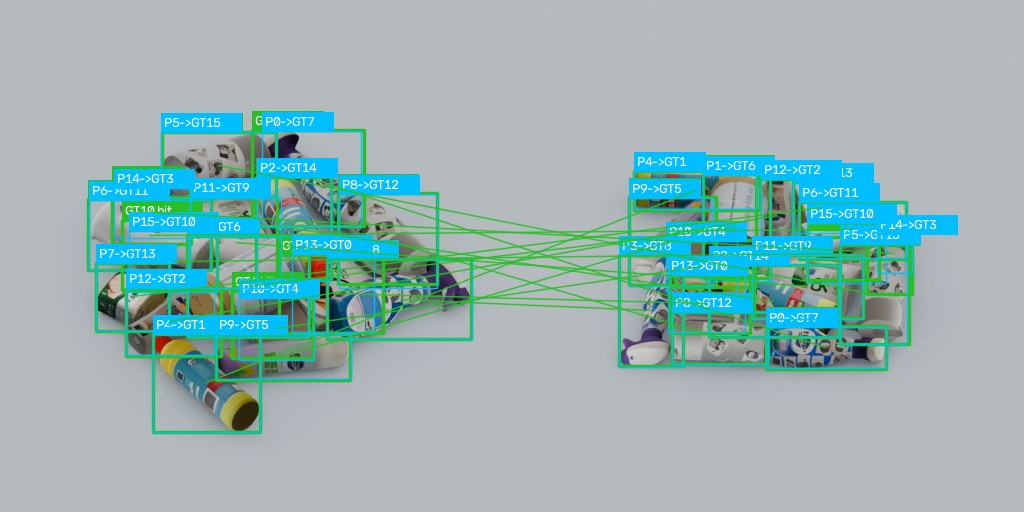
\includegraphics[width=\linewidth]{fig/scene_001001.jpg}\\[-1mm]
{\small (a) Clean example}
\end{minipage}\hfill
\begin{minipage}[t]{0.48\textwidth}\centering
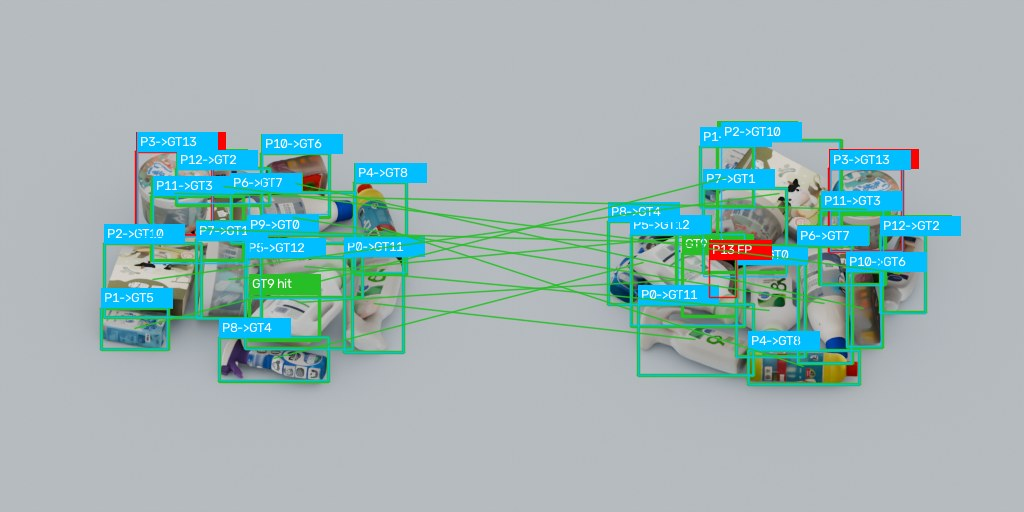
\includegraphics[width=\linewidth]{fig/scene_001000.jpg}\\[-1mm]
{\small (b) Misses and extra box}
\end{minipage}\hfill\\[2mm]
\begin{minipage}[t]{0.48\textwidth}\centering
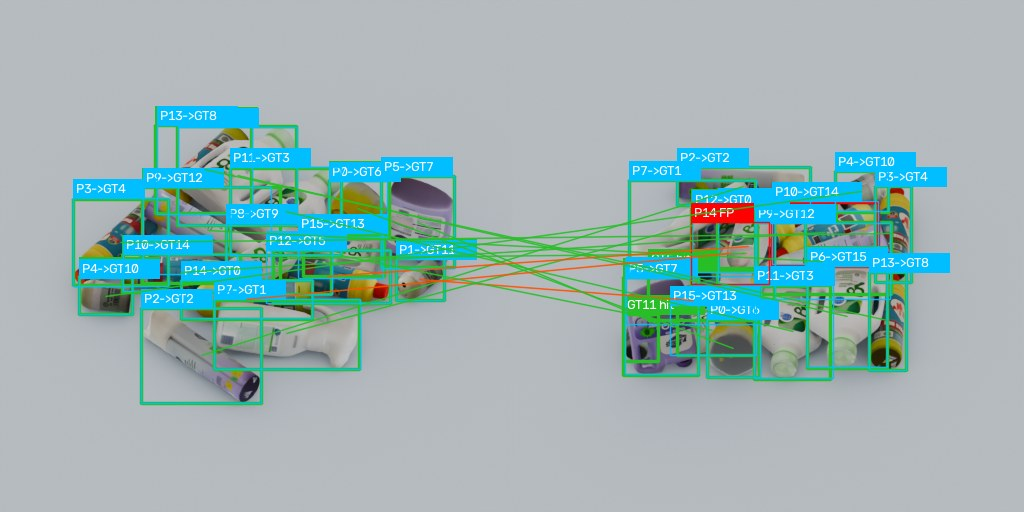
\includegraphics[width=\linewidth]{fig/scene_001002.jpg}\\[-1mm]
{\small (c) Wrong cross-view links}
\end{minipage}
\caption{Validation diagnostics from the selected scene matcher. Green outlines and links indicate correct matches; red and orange marks indicate detections or links that fail the evaluator's IoU-based matching. Each panel shows the two views of one scene.}
\label{fig:failures}
\end{figure*}

The 960-pixel detector with a learned scene-level matcher is the selected method because it gives the strongest measured balance of association and counting metrics. The experiment also shows that maximizing a single metric can be misleading: recovery marginally raises association F1, while the no-recovery model has lower count error and higher given-detection F1. Test predictions follow the required JSON structure and cover all 200 test scene pairs. Since test labels are withheld, no test accuracy is claimed. Future gains should focus on missed amodal boxes and ambiguous crowded-scene links without increasing duplicate records.

{
    \small
    \bibliographystyle{ieeenat_fullname}
    \bibliography{main}
}

% WARNING: do not forget to delete the supplementary pages from your submission 
% \input{sec/X_suppl}

\end{document}
